\section{Podstawowe ekrany}

W pierwszej kolejności opisane zostaną trzy podstawowe ekrany, które są obecne w obu aplikacjach. Są to ekrany powitalne, ustawień oraz podziękowań. Ich wygląd w aplikacji dla wykonawców został przedstawiony na rysunku \ref{fig:basic-expert}.

% \begin{figure}[ht]
%   \captionsetup[subfigure]{justification=centering}
%   \centering
%   \begin{subfigure}{0.32\textwidth}
%     \centering
%     \fbox{
\includegraphics[width=0.97\linewidth]{screens/splash_client.png}}
%     \caption{Ekran powitalny}
%   \end{subfigure}
%   \begin{subfigure}{0.32\textwidth}
%     \centering
%     \fbox{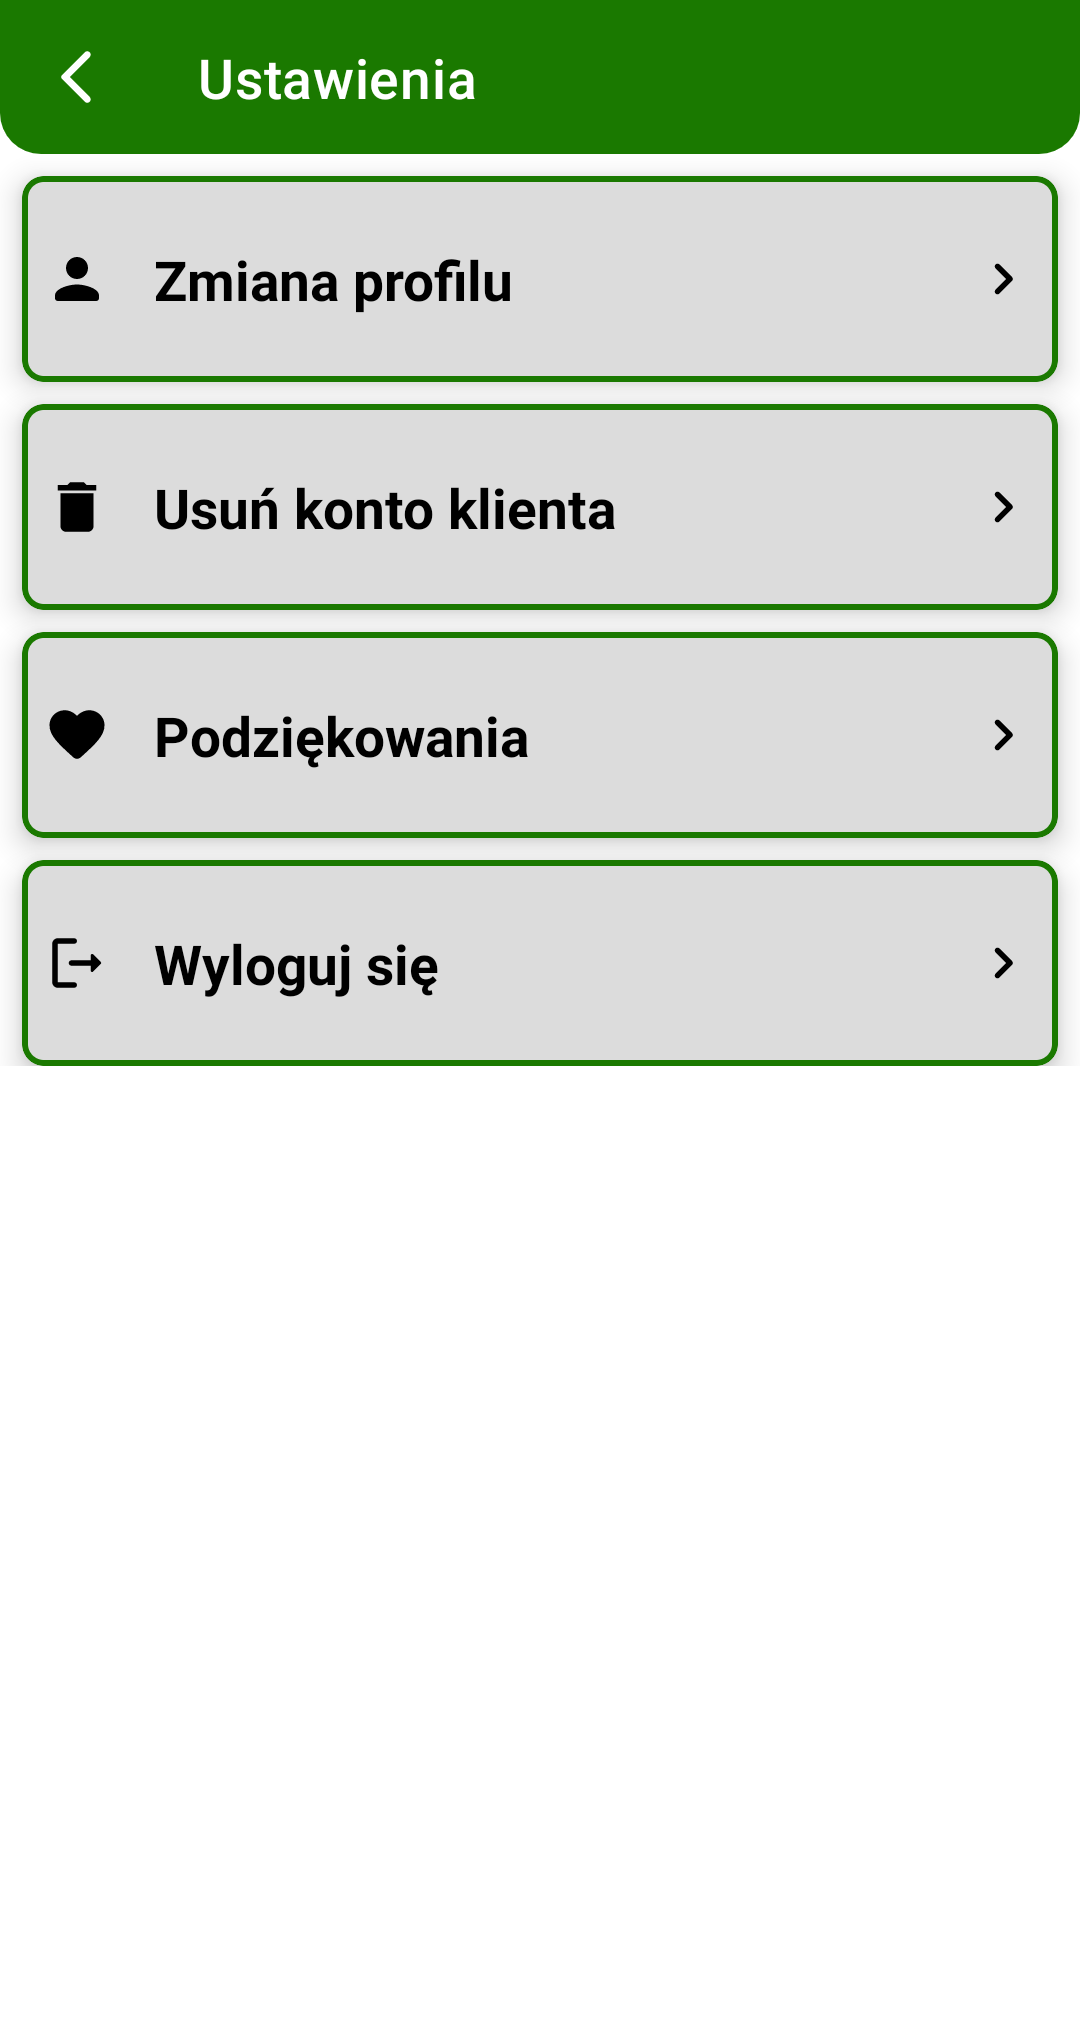
\includegraphics[width=0.97\linewidth]{screens/settings_client.png}}
%     \caption{Ekran ustawień}
%   \end{subfigure}
%   \begin{subfigure}{0.32\textwidth}
%     \centering
%     \fbox{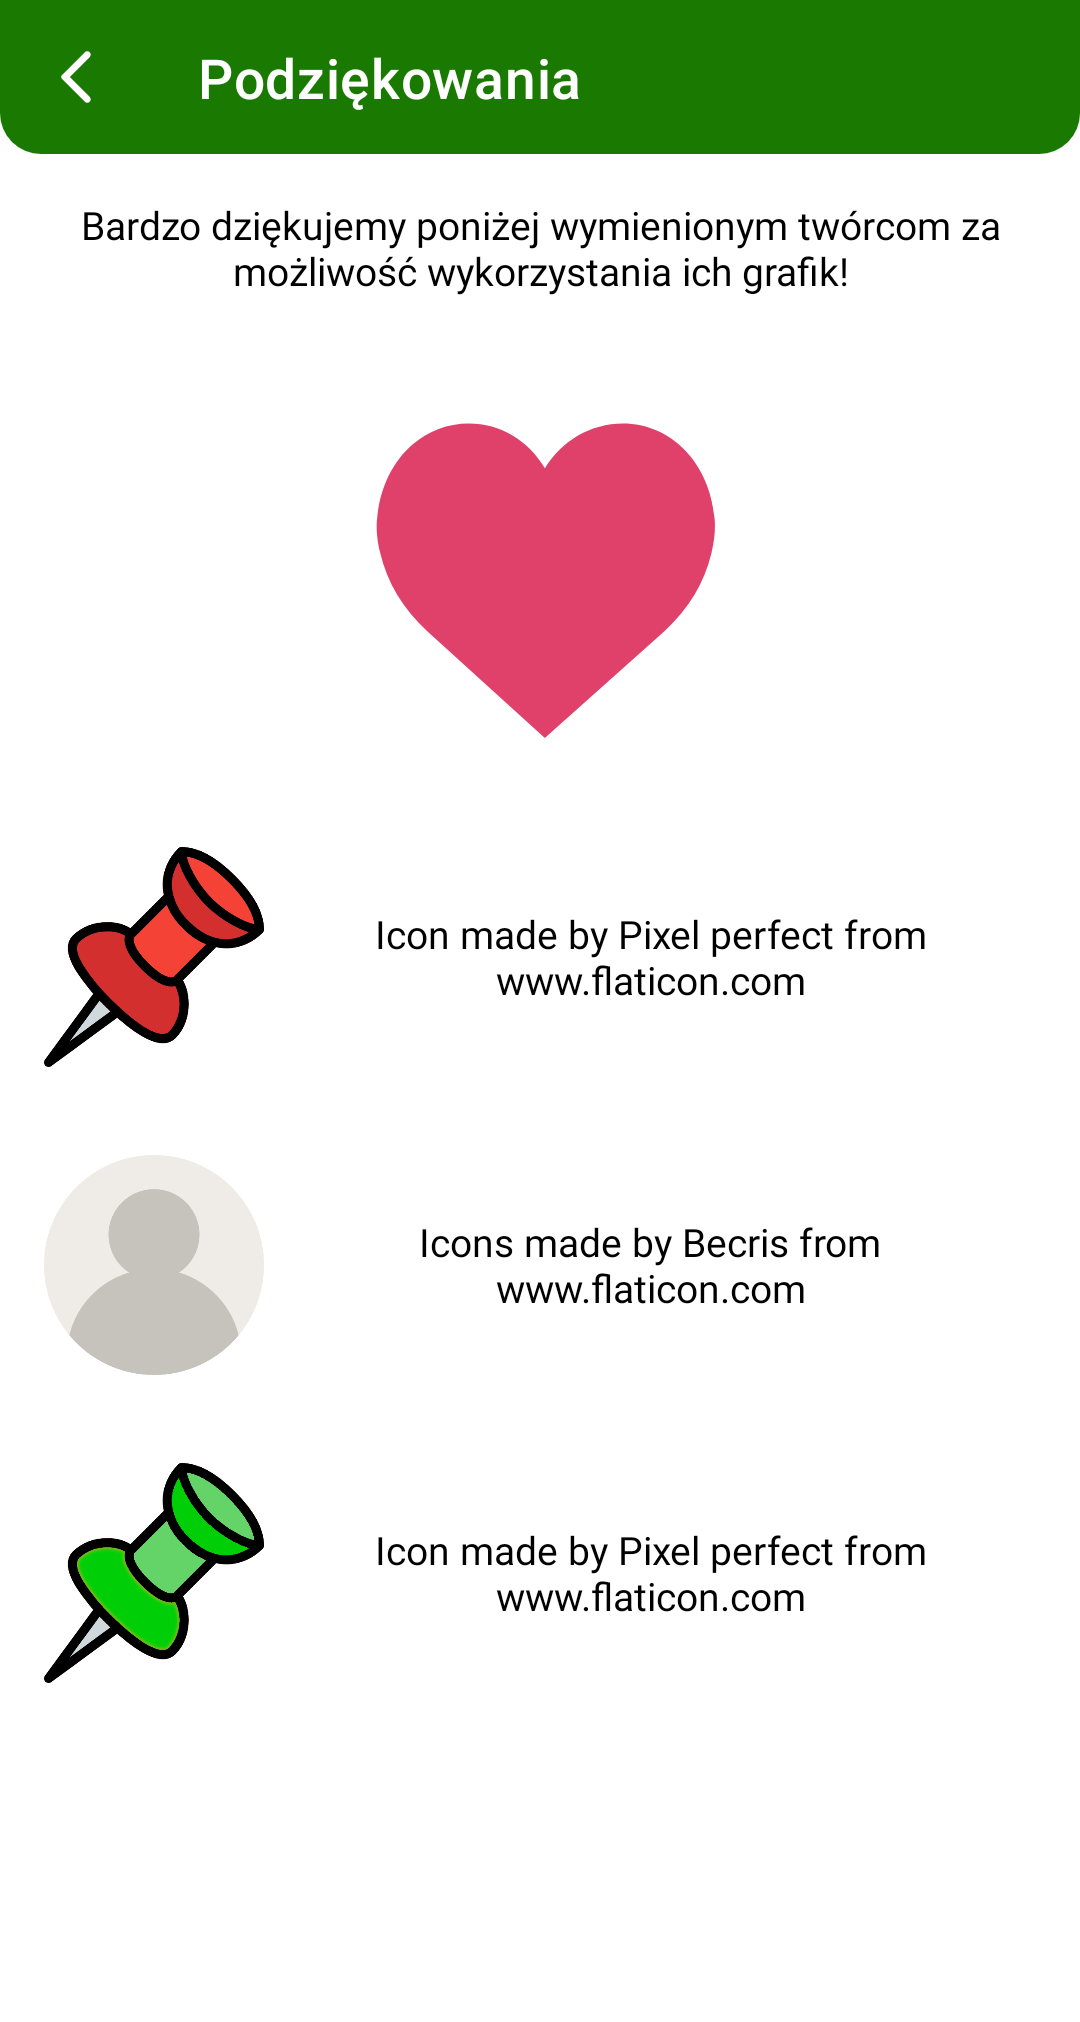
\includegraphics[width=0.97\linewidth]{screens/credits_client.png}}
%     \caption{Ekran podziękowań}
%   \end{subfigure}
%   \caption{Podstawowe ekrany aplikacji dla klientów}
%   \label{fig:basic-client}
% \end{figure}

\begin{figure}[ht]
  \captionsetup[subfigure]{justification=centering}
  \centering
  \begin{subfigure}{0.32\textwidth}
    \centering
    \fbox{
\includegraphics[width=0.97\linewidth]{screens/splash_expert.png}}
    \caption{Ekran powitalny}
  \end{subfigure}
  \begin{subfigure}{0.32\textwidth}
    \centering
    \fbox{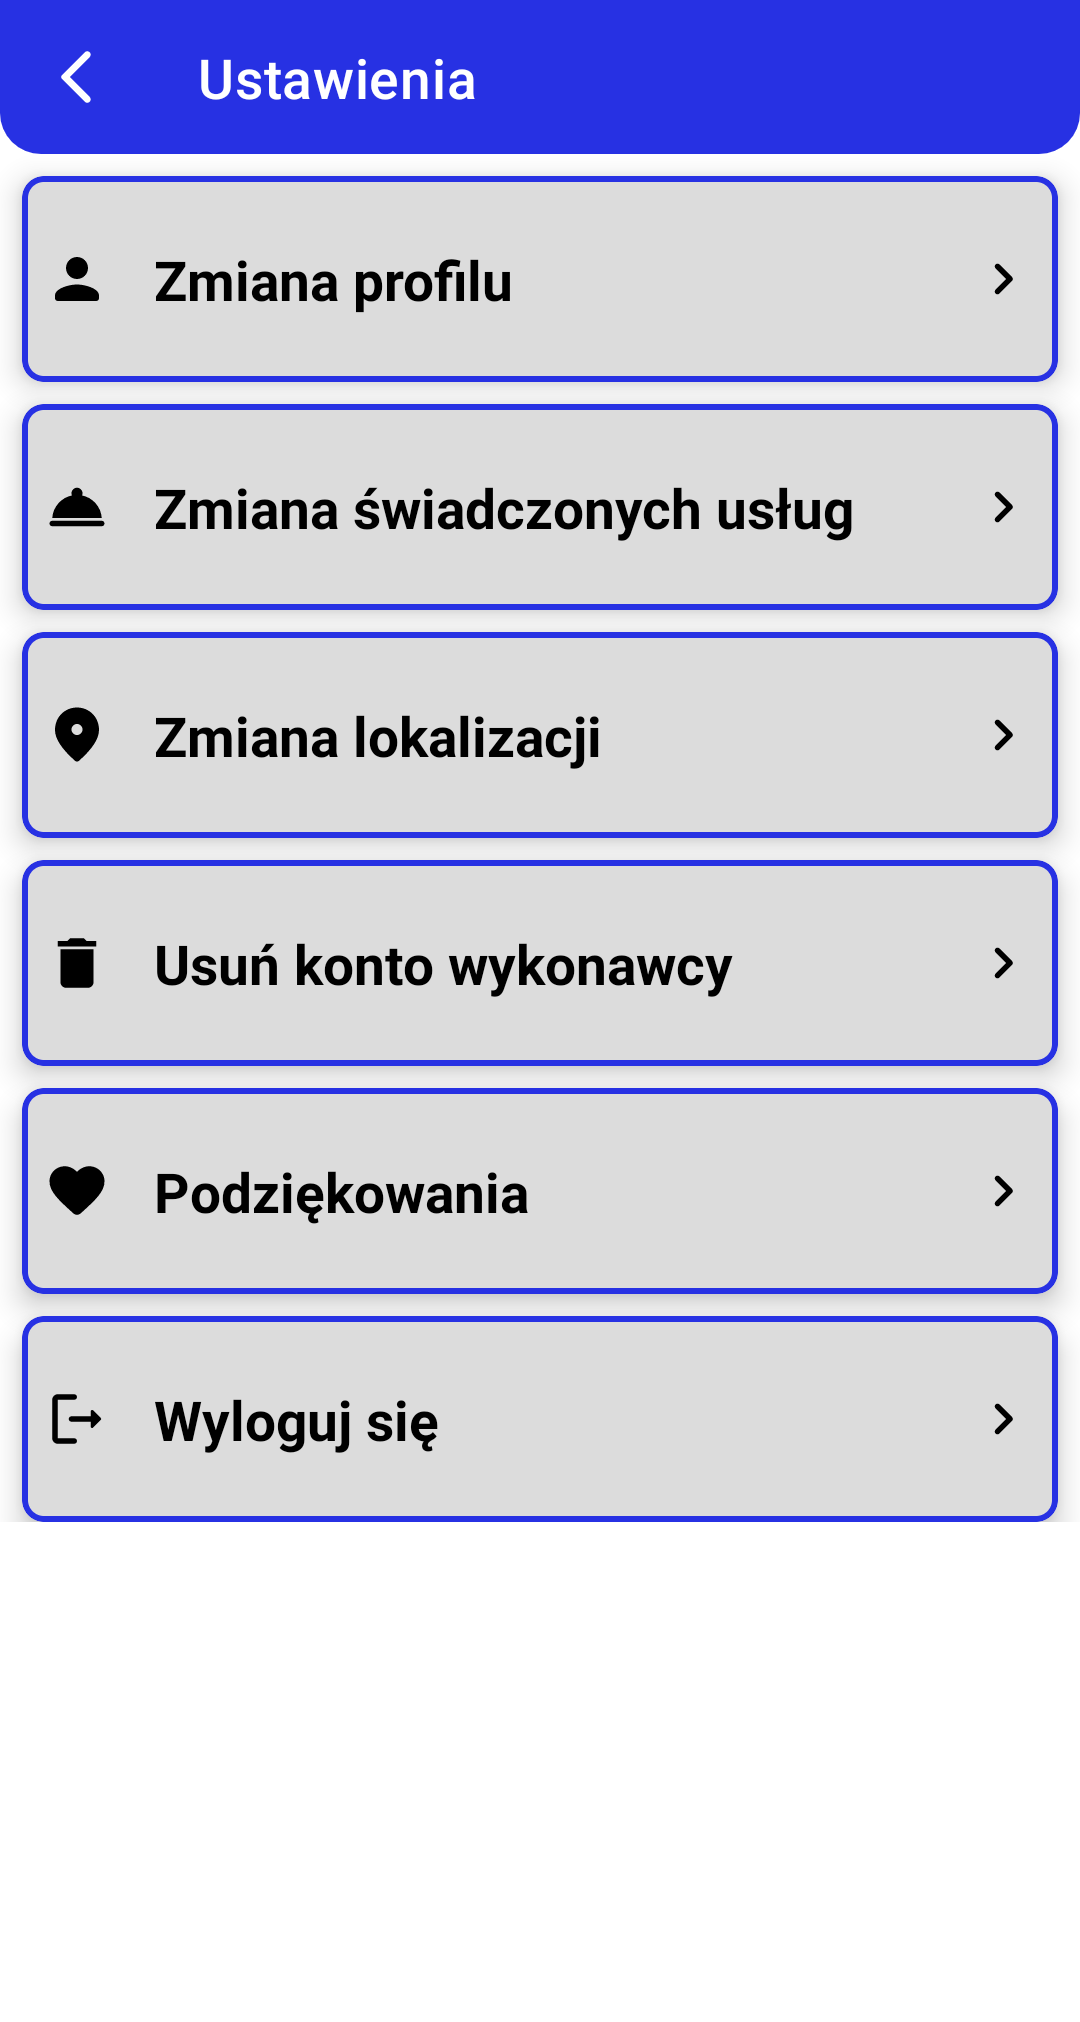
\includegraphics[width=0.97\linewidth]{screens/settings_expert.png}}
    \caption{Ekran ustawień}
  \end{subfigure}
  \begin{subfigure}{0.32\textwidth}
    \centering
    \fbox{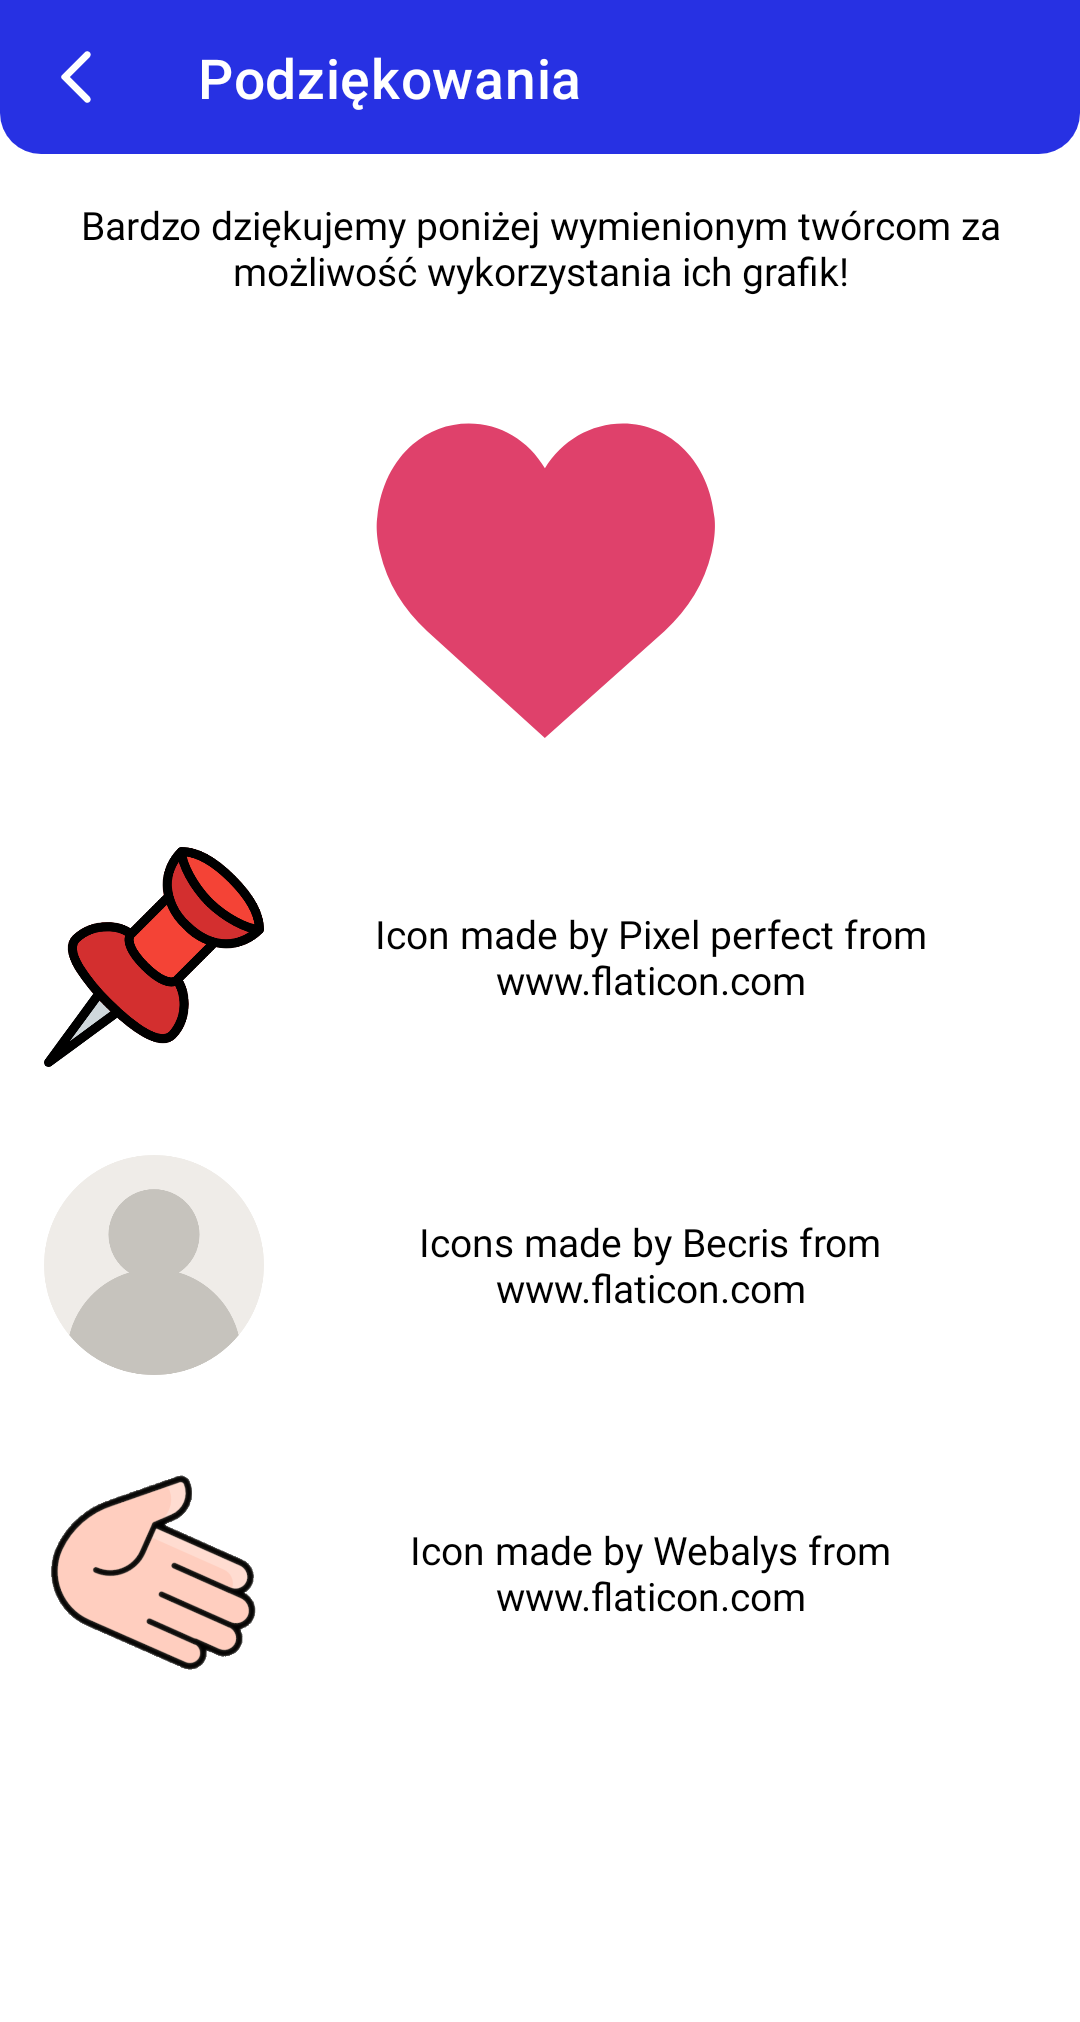
\includegraphics[width=0.97\linewidth]{screens/credits_expert.png}}
    \caption{Ekran podziękowań}
  \end{subfigure}
  \caption[Podstawowe ekrany]{Podstawowe ekrany w aplikacji dla wykonawców}
  \label{fig:basic-expert}
\end{figure}

Ekran powitalny, nazywany również często splash screen, jest widokiem wyświetlanym zaraz po uruchomieniu aplikacji. Została zastosowana w nim animacja, która stanowi przyjemny akcent. Podczas jej wyświetlania wykonywana jest logika określająca, który ekran powinien wyświetlić się jako kolejny. Jeżeli użytkownik nie jest zalogowany, to będzie to ekran logowania. Gdy już to zrobił, ale nie uzupełnił wszystkich wymaganych danych, to wyświetli się ekran, który to umożliwia. Jeżeli natomiast obie czynności zostały wykonane, to pokaże się ekran główny. Już tutaj widać dość skomplikowaną logikę, która dzięki wykorzystaniu trójwarstwowej architektury mogła zostać zamknięta wewnątrz przypadku użycia.

Ekran ustawień jest widokiem, którego głównym celem jest umożliwienie użytkownikom przechodzenia w inne części aplikacji. Znajdujące się w nim elementy różnią się dla wykonawców i klientów. Jedną ze wspólnych jest opcja umożliwiająca wylogowanie. Po jej wybraniu pokazywane jest okno dialogowe z prośbą o potwierdzenie.

Ekran podziękowań zawiera informacje o źródłach i autorach wykorzystanych grafik, jeśli tego wymagały. Znajdujące się tam wpisy dotyczą głównie ikon ze strony flaticon.com \cite{flaticon}, którymi postanowiono się posłużyć. W przypadku chęci ich bezpłatnego użycia podjęcie takiego działania zostało przedstawione jako konieczne.